\documentclass[a4paper,11pt]{article}
\usepackage[osf]{mathpazo}
\usepackage{ms}
\usepackage[]{natbib}
\raggedright

\newcommand{\datastorr}{\texttt{datastorr}}
\newcommand{\smurl}[1]{{\footnotesize\url{#1}}}
\newcommand{\ghsmurl}[1]{{\footnotesize\href{https://github.com/#1}{#1}}}

\usepackage{graphicx}

\title{Versioned data: why it’s needed and how it can be achieved (easily and cheaply)}
\author{Richard G. FitzJohn$^1$, Daniel S. Falster$^2$,\\ Matthew
  W. Pennell$^3$, and William K. Cornwell$^{2,*}$}
\affiliation{
$^1$ Imperial College, London, United Kingdom\\
$^2$ Evolution \& Ecology Research Centre, School of Biological, Earth and Environmental Sciences,\\
University of New South Wales, Sydney, NSW 2052, Australia\\
$^3$ Department of Zoology and Biodiversity Research Centre,\\
University of British Columbia, Vancouver, B.C. V6T 1Z4 Canada\\
$^*$ Corresponding author: w.cornwell@unsw.edu.au\\
}
\date{}

\bibliographystyle{mee}

\usepackage[title,titletoc,toc]{appendix}

\mstype{Article Note}
\runninghead{Versioned Data Delivery}
\keywords{}

\begin{document}
\mstitlepage
\noindent
\parindent=1.5em
\addtolength{\parskip}{.3em}
\doublespacing
\linenumbers


% For Analyses and Articles, the main text (excluding abstract, Methods, references and figure legends) is approximately 3,000 words. The abstract is typically 100-170 words, unreferenced. An Introduction is followed by sections headed Results, Discussion, Methods. The Methods and Results should be divided by topical subheadings; the Discussion does not contain subheadings. The Methods should be followed by References, Data Citations (optional), Acknowledgements and a Competing interests statement. A Data Citation section should be included when externally hosted datasets are referred to in the work and each can be cited formally with a unique, stable identifier and repository name.



\section{Summary}

Sharing data has become a key part of reproducible workflows in science.  To help this process, numerous linked tools have been developed to allow quick and easy data sharing.  Thus far, however, data has been largely considered a fixed and unchanging product---the particular data file for a particular analysis can be quickly unloaded, given a digital identifier, and shared.  While this is highly useful, this framework does not account for on-going scientific progress: for many important problems, epitomised by problems that lead to meta-analysis, datasets will continue to grow with time---more data points will be added, and new and more useful data structures will be created.  Essentially this means that data, like science in general, progress with time.  We suggest that a versioning system for data will facilitate this process.  Moreover, while the idea of versioned data has been taken up by large data sharing organizations, we present new tools for creating, archiving, and distributing versioned data easily, quickly and cheaply.  These new tools allow for individual research groups to shift from a static model of data curation to a dynamic and versioned model that naturally matches the scientific process.

\section{Introduction}

Data is now a first-class scientific product, as is evidenced by the advent of this journal \cite{Editorial-2014}. Increasingly, funding bodies, publishers, and scientific social norms are both requiring data to be published alongside research publications and recognizing the value of producing and sharing data without any accompanying analyses \cite[e.g.][]{Whitlock-2011,Fairbairn-2011,Piwowar-2011,VanNoorden-2013,Gibney-2013}. This has been a rapid, and exciting, sea change and the scientific community is still grappling with how best to disseminate data and credit data creators and aggregators \cite{Whitlock-2011, Goodman-2014, Lowndes-2017,Perkel-2016,VanNoorden-2013}. One thing that is clear is that there is no single best solution for managing and distributing data, as data types and use is incredibly heterogeneous. At one end of the spectrum are massive, centralized repositories that are constantly being added to; this is a great solution to storing and distributing relatively standardized data such as sequences (e.g., \texttt{GenBank}, \texttt{SRA}) (Table \ref{tab:sql_v_versioneddata}). At the other end are repositories for storing a wide variety of static, stand-alone datasets (eg. \texttt{Dryad}, \texttt{Figshare}, and \texttt{Zenodo}; or less optimally, as supplements to research papers)(Table \ref{tab:sql_v_versioneddata}). We suggest there is a substantial middle ground that is not well served by either of these existing paradigms, where a lightweight system for serving versioned datasets is needed.

In this article we i) introduce the concept of Versioned Data Delivery (VDD) and describe why it is needed; ii) outline how emerging technologies in data science (Table \ref{tab:technologies}) can be used to help researchers maintain, distribute, and access small-to-medium sized datasets; and iii) introduce a new R package called \texttt{datastorr}, an implementation of a VDD system. While we emphasize particular technologies in our implementation, the principles are general and could easily be ported to other platforms. While the examples cited here are in ecology and evolution; the issues identified and the solutions put forward are relevant to nearly all data-oriented scientific domains.

\subsection{Why versioning of data is needed and difficult}

Almost all useful databases are living--they \emph{should} get better
through time either by the addition of new data or by improving the
quality of existing data. For example a dataset on plant characteristics
might become outdated as taxonomic changes occur. Updating the dataset might only
require a small amount of work, but if there is no
way to distribute the updated dataset, then that work has to be re-done by
every user of that dataset. Moreover, those required changes add steps
between the canonical (or master) dataset and the new analysis (and publication),
making reproducibility of the new analysis more difficult than it needs
to be. If the canonical dataset is versioned--and versions are
accessible--the up-to-date data can be distributed, used, and analyses
based on any of the released versions data can be reproduced.  

While the benefits of versioned data are fairly clear, determining how to implement it has been contentious . The static model of data distribution widely used in science, where datasets are archived either as supplementary materials for a journal article
or under its own DOI, is simply not designed to provide streams of versioned
data (Table \ref{tab:sql_v_versioneddata}). A particular issue with the static
model is that data releases are mostly triggered by publication of academic
papers. But for a living dataset, there may be multiple releases made in
between papers. This is particularly the case with the discovery of small
errors. For any medium-sized dataset that is put to reuse, errors will
inevitably be found, and there needs to be some easy  way to correct them and
distribute the updated dataset.

To overcome the limitations of static datasets, many research groups have
setup dedicated webservers to host and distribute data. In these systems,
datasets areas maintained in a structure database, such as SQL, and a front
end to this database is written, often using a platform such as Ruby on rails.
When designed well, such systems are very useful for updating or adding to a
dataset. However, the infrastructure investment (designing maintaining, and
hosting the database) is clearly overkill for most projects and is a very
substantial barrier to entry. Furthermore, the system requires ongoing funds to maintain it, making it often unsustainable for many research groups. Moreover, the existence of a live webserver,
does not in itself guarantee ongoing access to different versions of a
dataset.

When considering the right tool to store and deliver versioned data, the size
of the dataset is another essential consideration. ``Big data'' brings with it
specific needs and so requires a specific set of hardware and software tools.
Examples of big data include genetic datasets, global datasets of species
observations, and remote sensing data. This size of this data is bigger than
that which individual research groups can maintain and often requires a
specialized governmental or non-governmental institution with full-time staff
to curate and maintain those research resources. Here we are particularly
interested in smaller and more specialized problems (e.g., cases where a single 
research group contributes most of the data). In most of these cases, the data
collected will not be ``big'' but rather small-to-medium sized. Such data
support research projects, but are not in most cases general enough to
establish bespoke infrastructure for. But crucially the data themselves will change
over time. And currently there is no infrastructure for organizing and
distributing these types of ``living datasets''.

So what is needed is simple tool-chain for
making versions of a dataset and delivering it to potential users, along
with notes on what has changed and why since the previous version.
Table \ref{tab:user_requirements} outlines what we consider requirements for
three groups of people interacting with this system: maintainers,
contributors, users. The solution is ideally low-cost (both in money and
time), sophisticated, yet requiring little skill to setup and use.  Ideally
there would also be a way for users to also become contributors, by flagging
errors for the curator to correct in the next release, or even for the user to
fix themselves.

% For small datasets, it is simply not possible to use the same tools developed for
% big data: there are a number of high-setup-cost options (stand-alone
% websites, APIs), which have advantages if you have the resources to
% develop and maintain them. We wanted a relatively low cost way (both in
% money and time).

\section{Results}

\subsection{A lightweight, cheap and scalable workflow for versioned data}

% DF: Bring out general features more. Right now git delivers this. With the growth of open-source tools and collaborative platforms, we believe all the features needed for delivering the vision outlined above are now present. The workflow we describe below builds off existing platforms and combines them in new ways, and offers the potential for widespread uptake at little or no cost.

In brief, the workflow we present, which we call Versioned Data Delivery (VDD), borrows best-practices for software development \cite{Perez-Riverol-2016} and applies them to the challenge of maintaining and distributing versioned data. Software developers maintain a core set of code which produces a binary executable file that can be installed on a users local  computers. With a VDD system, data developers maintain a core set of files, which produce an organised dataset that can be similarly be ``installed'' on a user's local computer. In either the development of software or data, successive versions are released over time (called ``releases''). The similarity in workflow between software and data then allows us to deploy the same technological platforms that are used in software development, for the development and distribution of data. Importantly, VDD uses well-established tools, ensuring high-level performance and stability.

The core technologies used are summarised in Table \ref{tab:technologies} and described further below.

\subsection{Version control}

Version control, primarily an open-source variety called \texttt{git}, has become ubiquitous in software development.  Essentially version control tracks line-by-line changes in text files and creates and maintains a history of those changes. Increasingly version control has been applied to scientific code and data management, especially for small-to-medium sized datasets \citep{Ram-2013, Perkel-2016}. Git is attractive for data management because it tracks all changes in monitored files. This history is visible to anyone interacting with the repository. It also allows users to annotate changes (`commits') with informative messages detailing the rationale for those changes.
  
Because \texttt{git} was built for tracking changes in code, there are aspects of how it behaves that are not natural to apply to  data \cite{Perkel-2016}.  For example, because it tracks changes line-by-line rather than cell-by-cell, there are inefficiencies in how the software stores the changes.  There is rapid current work on this problem and prototypes available, and as such, it is likely that \texttt{git} for data will replaced by a more natural system for data in the near future  \citep{Fli, Dat}.  This future system would be faster computationally, smaller in file size, flexible with respect to data structures, and thus allow for larger datasets to be versioned efficiently.  That said, the workflow we describe here currently works well with \texttt{git} and should work even more quickly with its future replacement.

\subsection{Cloud platforms for storing and distributing version controlled data}

There are many current platforms for storing and distributing versioned controlled data for low or no cost.  The website GitHub (\smurl{www.github.com}) is a commercial platform for hosting and interacting with git repositories. In practice, each dataset should be a separate git repository on github (see Table \ref{tab:examples} for examples). Although mainly used for computer code, Github is now also being use to manage scientific data \citep{Perkel-2016}. Maintaining the version controlled data in the cloud has two main benefits: first, it provides a platform for multiple data contributors to sync their files and correspond about changes in the dataset, and second, it hosts a stream of data releases, thus acting as a central point for  the collection, curation, and distribution of the data.

\subsection{Potential for collaboration: allowing for one or more data contributors}

\textbf{Pull requests}: Much of the activity on GitHub is on open-source projects with many contributors. An essential feature that of sending a pull request, whereby a would-be contributor submits prospective changes to be incorporated.

\subsection{Cloud platforms for storing and distributing version controlled data}

There are many current platforms for storing and distributing versioned controlled data for low or no cost.  The website GitHub (\smurl{www.github.com}) is a commercial platform for hosting and interacting with git repositories. In practice, each dataset should be a separate git repository on github (see Table \ref{tab:examples} for examples). Although mainly used for computer code, Github is now also being use to manage scientific data \citep{Perkel-2016}. Maintaining the version controlled data in the cloud has two main benefits: first, it provides a platform for multiple data contributors to sync their files and correspond about changes in the dataset, and second, it hosts a stream of data releases, thus acting as a central point for  the collection, curation, and distribution of the data.

\subsection{`Semantic' versioning}

To fully realize the benefits of a versioned data, the VDD system needs to be communicated to the user.  Crucially a user should be immediately aware of the relationship among versions.  Software development has dealt with a very similar problem, and we suggest there is benefit in adopting the notation from that field.  Specifically, we suggest applying the theory of ``semantic versioning'' developed for software distribution. This system uses (the potentially familiar) notation of form ``1.0.0'' for successive versions (Fig \ref{fig:semantic}). As has been noted (REFS), labelling of data versions presents a similar problem to the labelling of software releases: signalling to users the types of change that has occurred between successive versions. Applying semantic versioning to data, a change from 1.0.0 to 1.0.1 implies tiny changes, for example a minor error correction. A change from 1.0.0 to 1.1.0 implies a substantial enhancement, for example adding a new study to a meta-analysis dataset (while otherwise maintaining the same dataset structure). A change from 1.0.0 to 2.0.0 implies a very major revision, for example improving the entire structure of the dataset and adding new columns.

\subsection{Digital object identifiers}


Tools for creating and archiving digital objects have seen rapid progress in recent years.  At present, each version of the dataset can be automatically archived and assigned a DOI, via several providers (Table \ref{tab:doi_minting}).  Here we describe the particular integration of github and zenodo.  It is useful to have the ability to either be specific---reference a parti

TODO: FLESH THIS OUT AND ADD REFERENCE TO BLOG POST AND OTHER THINKING ON THIS


\subsection{Distributing data to different user needs}

At current there are two classes of data users: those that  interact with the data via point and click downloading and those that use code-based interaction.  The system we describe allows for both types (Figure \ref{fig:technology_stack} and Table \ref{tab:user_requirements}).  GitHub has a feature called ``releases'' in which specific commits can be turned into a version for distribution (with associated version number).  Those releases can be downloaded directly by users via point-and-click, or accessed via the Github API. Releases can also be embedded into any kind of website that allows the data curator to facilitate discovery by more users and to provide context.  Releases can also be linked to code-based users via an R package which we describe in the following section.

\subsection{\texttt{datastorr} and dataset-specific R packages}

A point-and-click workflow may create barriers for reproducibility \cite{Wilson-2014,Lowndes-2017}. Ideally, users should be able to also able access the all versions of the database programmatically. To this end, we offer a novel implementation of a VDD system. We have written a R package, \texttt{datastorr} (\smurl{github.com/richfitz/datastorr}), that a) interacts with the GitHub API to pull down versions of the dataset; and b) constructs the shell of a second, database specific R package, which can be used to access versions of the dataset. Using this system, a researcher can create and distribute a R package that facilitates access to her data with (very) minimal computational skills.

For example, \texttt{datastorr} was used to build the package \texttt{baad.data} (\smurl{github.com/dfalster/baad.data}), which is an interface to the Biomass and Allometry Database (BAAD) stored at \smurl{github.com/dfalster/baad}. \texttt{baad.data} consists of only a few simple functions, that were automatically generated (along with the associated help files) with \texttt{datastorr}. And importantly \texttt{baad.data} contains no actual data so is very quick to install and takes up virtually no space on the user's harddrive. When the function \texttt{baad.data::baad\_data()} is called, the system will download the latest version; if there have not been any changes since the last time the function was called, it will simply retrieve the data from memory, making the system very efficient (and also allowing the system to work seamlessly if the computer is offline). If a researcher requires an older version of BAAD, perhaps to reproduce an analysis, specifying the version number of the data as an argument in \texttt{baad.data::baad\_data()} will retrieve and store this, without overwriting any other dataset versions they may have previously downloaded.

Using \texttt{datastorr}, researchers can set up their own versioned database (and R package) simply by providing: 1) a github repository name (e.g., ``traitecoevo/taxonlookup''); 2) a single file that will contain the versioned data (e.g., ``taxonlookup.csv''); 3) and the function used to load this into \texttt{R} (e.g., \texttt{read.csv()}). A tutorial explaining precisely how to set this up is available at \smurl{github.com/richfitz/datastorr}. % is this the right site?  ropensci?

Then as the data changes (and hopefully improves) with time, update the data
file and create a github release with a new version number (preferably
using \href{http://semver.org/}{semantic versioning}). All the versions
will be available to the user. 

We have created \texttt{datastorr} to make VDD easy to implement and manage for \texttt{R} users. And as we stated above, this has already been used to release a variety of datasets (Table \ref{tab:examples}). However, we can imagine alternative methods for interacting with GitHub and building templates and adopting a VDD system does not critically depend on using \texttt{datastorr}. Indeed, we would love to see implementations in \texttt{Python} or other languages.

\section{Discussion}
% General problem. An example of solution. Key features

The problem of tracking data through time and versions is likely to be widespread. There are many alternate solutions, with associated features and drawbacks.  The current structure of scientific research is very distributed, with research groups across the world working on the same question.  Moreover at a time of funding scarcity, many world-class research groups do not have excess funds to hire and support technology specialists.  As such we argue that there is a niche for a easy, cheap, and flexible VDD system.  

Many of the key roadblocks preventing a switch from a static to a dynamic data world, were technological: in the past it took great deal of money and expertise to set up a VDD system. The proliferation of cloud--based tools and open--source software have now reduced these roadblocks considerably.  We argue that by linking together the tools described above, researchers can now produce, curate and distribute versioned data much more easily and cheaply than in the past.  

The key features of a VDD system that are already possible are a versioning system to communicate small and large changes to users, both point-and-click and code-based access to all versions, reliable distribution to many users, and stable, organized DOIs.  Moreover, it is relatively easy to update and add new versions.  Technology is moving forward rapidly and so it is very likely that the particular tools we describe above will add features and be even easier to use.  But, nonetheless, workable systems are already possible.  



%Topics to consider:
%
%\begin{itemize}
%
%\item Addresses important need, using open source platforms. Shows power of open source: by writing single new package, can provide global distribution and access to data, with first class system for managing contents.
%\item Versioning and open access essential for reproducibility
%\item Versioning should enable better benchmarking of models, also because tests can be automated.
%\item We have focussed on particular set of tools, but could do similar things with other platforms or languages.
%....
%\end{itemize}



%(old content unchanged)
%
%One of the key problems in switching from a static to a dynamic data
%world, is that it's currently hard to set up and maintain a system like
%this. Ideally using a versioned database should be easy for both the
%user and the data maintainer. This is especially crucial is the data
%maintainers are busy. Moreover, old versions need to be preserved in a
%stable and accessible way.
%
%To try and achieve to above goals, we built a system to distribute
%versions of our datasets. We think that with this infrastructure, it is
%relatively easy to set up and maintain a versioned system with any
%small-to-medium sized dataset.
%
%In our system, the data is downloaded only once per computer, available
%for offline access, easy to port to other platforms, and can get a doi
%when desired (i.e.~when it's used for a publication). All old versions
%are accessible.
%
%
%
%\subsection{How much expertise is needed to setup and use?}
%
%To use a versioned dataset: Very very basic \texttt{R}. With 4 lines of \texttt{R} code, you can
%have the data downloaded and loaded into R and ready for use.
%
%To set a system like this up: Basically there are two general skills required: 1) understanding
%version control via \texttt{git} and 2) writing a very simple R package.
%From the prolific Hadley Wickham there is a
%\href{http://r-pkgs.had.co.nz/git.html}{very clear introduction to git}
%and \href{http://r-pkgs.had.co.nz/intro.html}{an instruction to the
%basics of R packages}.


\subsection{Conclusion}



\newpage

\section{Tables}

\begin{table}[h!]
\centering
\caption{Alternative frameworks for setting up and managing a living database}
{\footnotesize
\vspace{1cm}
  \begin{tabular}{p{2.5cm}p{3.5cm}p{3.5cm}p{4cm}}
  \hline
  \textbf{Feature} & \textbf{Static datasets}& \textbf{Web database} & \textbf{Lightweight versioned data}\\
  \hline
   Webserver        & e.g. dataDryad & custom                          &  Maintained by github.com\\
   Backend          & none & SQL + Ruby-on-rails 			& git + datastorr \\
   User access      & Web browser & Web browser 				    & R \\
   Ease of setup    & Very easy & Hard 							& Easy\\ % server, backups, bandwidth
   Data size        & Up to several Gb & Small-Very large 				& Up to 1Gb\\
   Cost             & Varies & Varies  						& Free \\
   Bandwidth        &managed by dataDryad & Pro rata 						& Managed by github.com\\
   Maintainer skills &none & Ruby + php 					& R + git \\
   User skills      &Web browsing& Web browsing  					& basic R \\
   Versioning       &None& Hard 							& Easy \\
   DOI minting      &Automatic & Many steps 					& Automatic \\
  \hline 
  \\
 
  \end{tabular}
  } 
\label{tab:sql_v_versioneddata}
\end{table}

\newpage

\begin{table}[h!]
\centering
\caption{Technologies used to maintain, store and distribute "Lightweight versioned data".}
{\footnotesize
\vspace{1cm}
  \begin{tabular}{p{5cm}p{10cm}}
  \hline
  \textbf{Technology} & \textbf{Description} \\\hline
   git & Open source version control system used for tracking progressive changes in a set of text files, typically computer code but also data\\
   github.com & A commercial webplatform for sharing, visualising and managing `git' repositories. Includes issue tracking\\
   R     &  Open source statsitcial and data processing language \\
   CRAN  &  Open source repository of packages for the R language \\
   datastorr & R package used to fetch versioned releases from github  \\
   DOI & Digital object identifier, which refers a user to a single stable digital object \\ 
   DOI ``minting'' & creation of a DOI's \\
   \hline
  \end{tabular}
  }
\label{tab:technologies}
\end{table}

\newpage

\begin{table}[h!]
\centering
\caption{Groups of users and their requirements}
{\footnotesize
\vspace{1cm}
  \begin{tabular}{p{2cm}p{5cm}p{7cm}}
  \hline
  \textbf{Group} & \textbf{Goal} & \textbf{Requirements} \\ \hline
  Maintainer & Create and distribute versioned datasets & Low technical overhead \\
    & & Easy workflow for releasing new versions \\
    & & Long term preservation \\
    & & Easy to crowd-source error checking and contributions \\
    & & Low initial cost \\
    & & Low on-going maintenance \\
  Contributor & Contribute to future versions & Add new data \\
    & & Report errors in existing data  \\
  Users (all) & Easy access to releases & Introduction \& overview \\
    & & Long term stability \\
    & & Clear path for users to become contributors \\
  Users (computational, machines) & Build reproducible products on these data & Scripted access to releases\\
    & &Easy installation\\
    & & Long term stability \\
  \hline
  \end{tabular}
  }
\label{tab:user_requirements}
\end{table}

\newpage


\begin{table}[h!]
\centering
\caption{Alternative platforms for minting DOIs from github repositories}
{\footnotesize
\vspace{1cm}
  \begin{tabular}{p{4cm}p{8cm}}
  \hline
  \textbf{Provider} & \textbf{Features} \\ \hline
  Zenodo: \smurl{zenodo.org} & Automated DOI for each github release \\
    & Funded and maintained by CERN and OpenAIRE for long term preservation \\
    & Only includes files embedded in git repo, not built  by code\\
  Figshare: \smurl{figshare.com} & Builds data package based on github release \\
    & Allows you to upload additional files, e.g. datasets built by code \\
    & Integrated with several journals, e.g. Nature family, PNAS \\
    & Some limited potential for versioned DOIs\\
  \hline
  \end{tabular}
  }
\label{tab:doi_minting}
\end{table}

\newpage

\begin{table}[h!]
\centering
\caption{Example datasets using the lightweight versioned data workflow described in this paper.}
{\footnotesize
\vspace{1cm}

  \begin{tabular}{p{3.5cm}p{3cm}p{7cm}}
  \hline
   \textbf{Github repo} & \textbf{R package} & \textbf{Description} \\ \hline
  \ghsmurl{dfalster/baad/} & \texttt{baad.data} & The \texttt{Biomass And Allometry Database} \citep{Falster-2015} provides...\\
  \ghsmurl{traitecoevo/taxonlookup} & \texttt{taxonlookup} & \texttt{taxonlookup} \citep{Pennell-2015a} provides...\\
  \ghsmurl{github.com/...} & \texttt{fungaltraits} & \texttt{fungaltraits} (in progress) provides... \\
  \hline
  \end{tabular}
  }
\label{tab:examples}
\end{table}

\newpage
\section{Figures}

\begin{figure}[!hb]
\centering
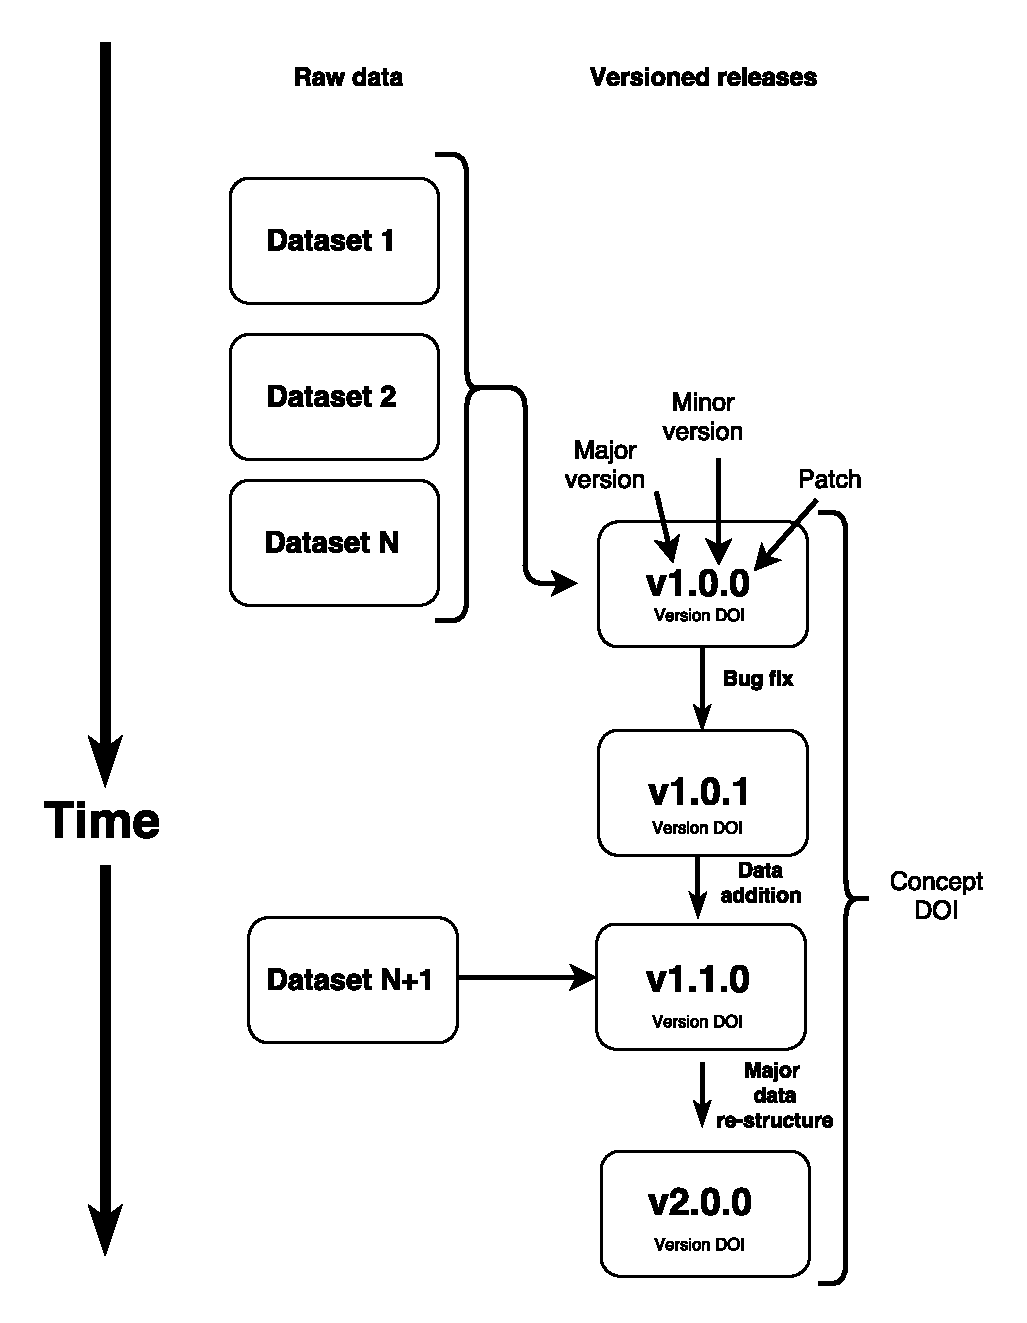
\includegraphics[width=\linewidth]{figures/Figure1.pdf}
\caption{Semantic versioning allows users to anticipate the types of changes that have occurred between successive versions of a dataset.
\textbf{a)} 3 numbers indicate type of change.
\textbf{b)} A typical release stream.}
\label{fig:semantic}
\end{figure}

\newpage


\begin{figure}[!hb]
\centering
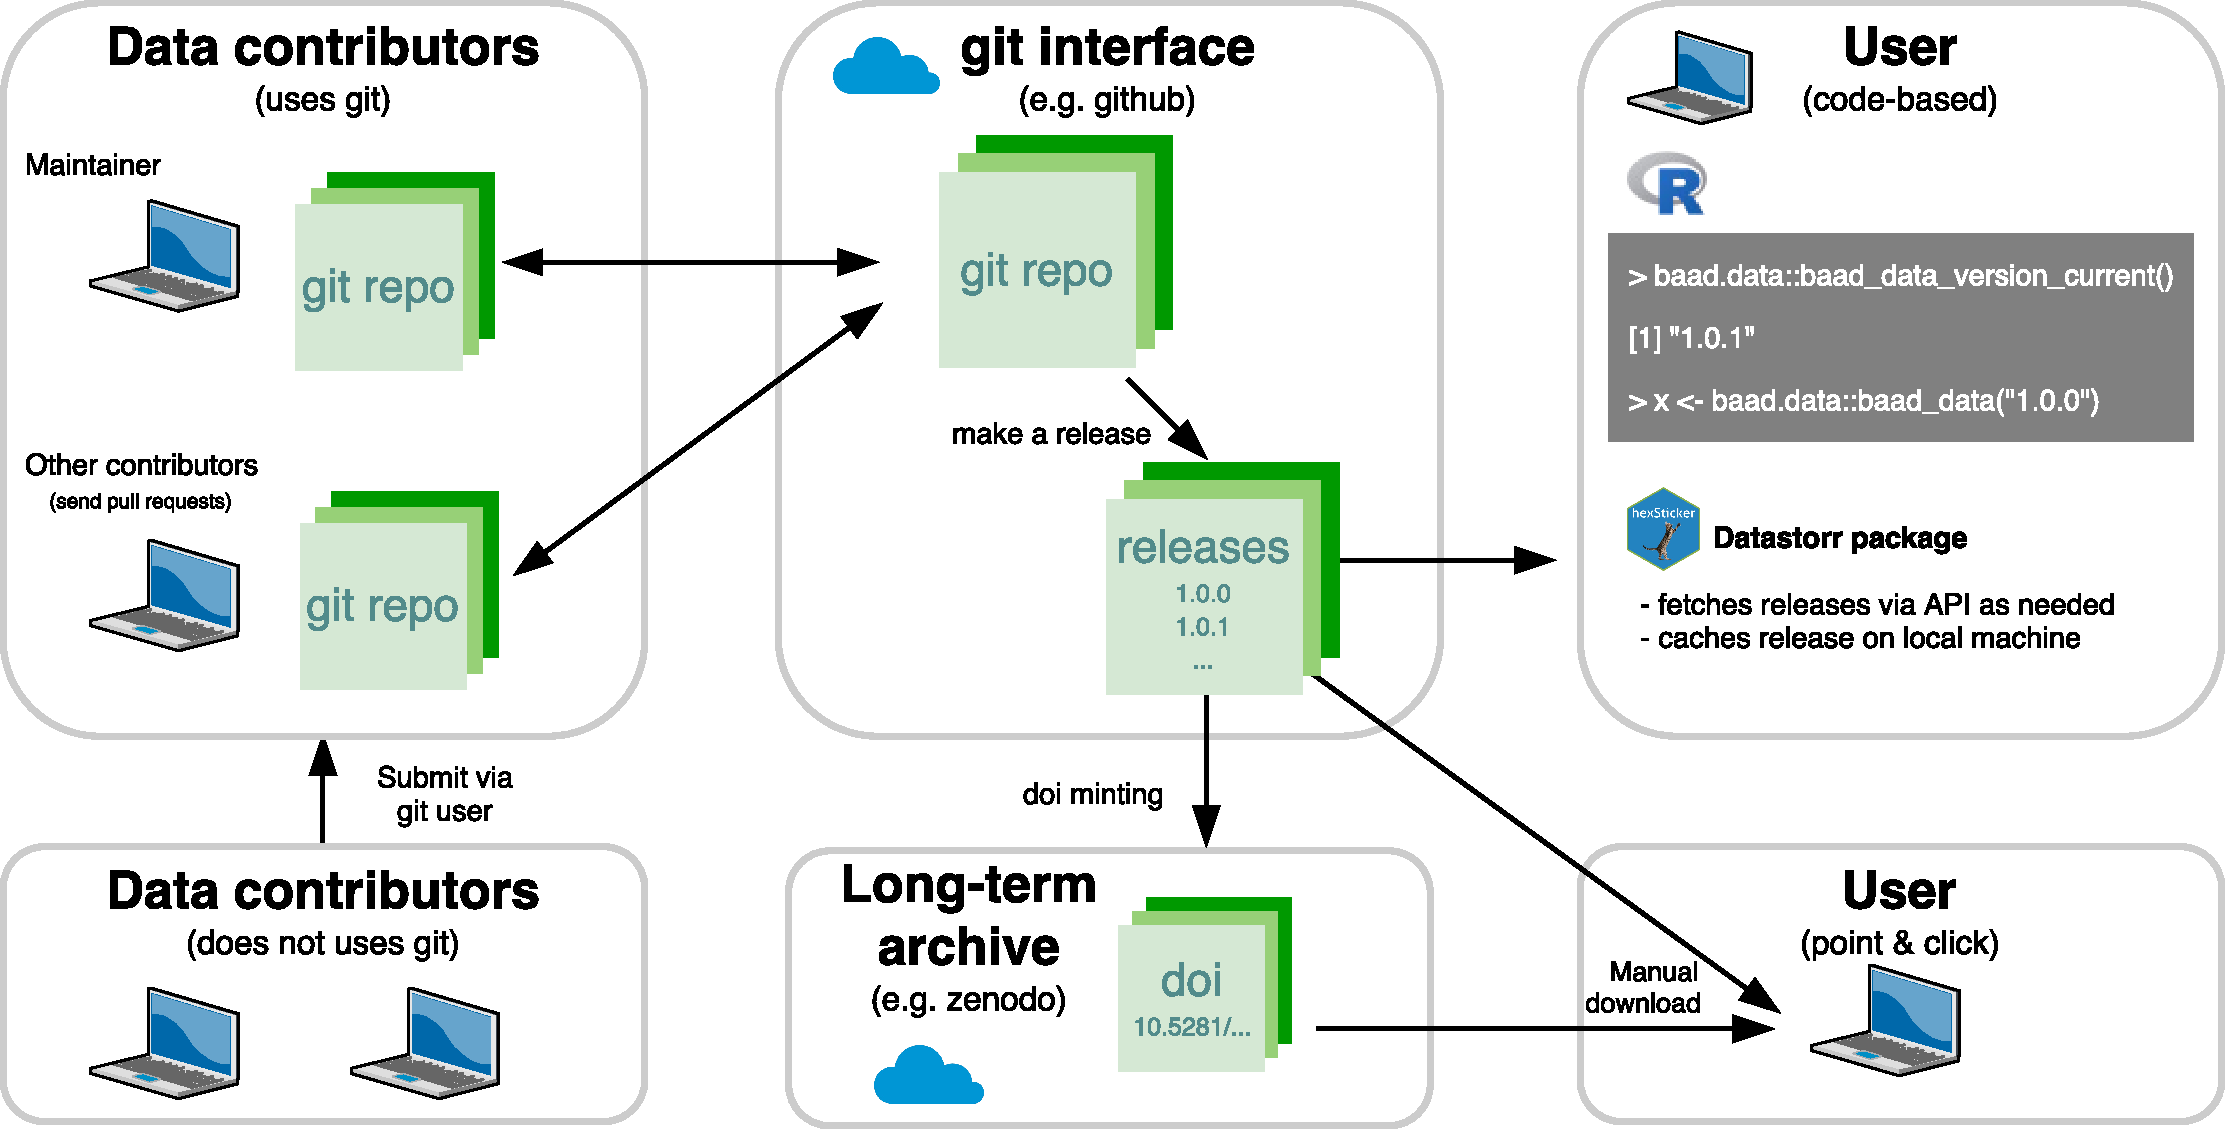
\includegraphics[width=\linewidth]{figures/Figure2.pdf}
\caption{Overview of the technologies involved in distributing versioned data via datastorr.}
\label{fig:technology_stack}
\end{figure}
\bibliography{refs}

\end{document}

